\section{Implementering}

\subsection{Hostname}
For at udskrive hostnavnet på maskinen i shell'en, har vi åbnet filen "/proc/sys/kernel/Hostname" med fopen(). Derefter læser vi første linje i filen ind i en buffer med fgets(), og scanner linjen ind i vores hostname variabel med sscan(). Til sidst lukker vi filen med fclose(). Der er ikke nogen fejlhåndtering, hvis filen ikke indeholder noget, eller hvis den ikke eksisterer. Begrundelsen for, at vi ikke fejlhåndterer her, er, at vi initialiserer vores hostname variabel med strengen "DEFAULT" og derefter overskriver denne variabel. Hvis filen ikke eksisterer, bliver hostname ikke overskrevet, og shell'en vil altså udskrive "DEFAULT".

\subsubsection{Valg af exec funktion}
Vi valgte først at afgrænse de mulige eksekveringsfunktioner til de tre, der understøttede automatisk opslag efter eksekverbare filer i de filkataloger, der er specifiseret i PATH miljøvariabelen. Disse er execlp(), execvp() og execvpe(). Dette gør det let at køre kommandoer som ls og wc.

Funktionen execvpe() blev udelukket, fordi den understøtter ekstra funktionalitet, som vi ikke har brug for i form af muligheden for at specifisere miljøet for kommandoen, der eksekveres.

Forskellen på execlp() og execvp() er kun formateringen af argumenterne, og her foretrak vi execvp(), fordi vi har brugt den før.
Alle funktionerne benytter sig alligevel i sidste ende af execve().

\subsection{Baggrundskørsel af kommandoer}
Vi har implementeret to forskellige måder at køre kommandoer på. Det er implementeret i de to metoder foregroundcmd() og backgroundcmd(), der begge er at finde i forback.c. Foregroundcmd forker hovedprocessen, og får forælderprocessen til at vente på at barneprocessen terminerer, dette er hvad vi kalder en forgrundsproces. 
Backgroundcmd forker hovedprocessen. Hovedprocessen venter på barneprocessen, mens barneprocessen igen forker sig selv og ekskvere kommandoen, uden at vente på den. Der forkes to gange for at undgå, at baggrundsprocessen ender som en såkaldt zombieproces, efter den terminerer.  

\subsection{Exit kommando}
Afslutning af shell'en sker, når brugeren skriver "exit" i kommandolinjen. I filen bosh.c findes metoden executeshellcmd(), hvor der foregår et check af kommandoerne. Hvis den første kommando er "exit", så returner executeshellcmd() tallet 1 til den kaldende metode, main metoden. Her bliver terminate-variablen sat til 1 og while loopet, der holder shell'en kørende, ved at chekke om terminate IKKE er 1, vil slutte.

\subsection{ctrl+c}
Ctrl+c sender et SIGINT-signal til shell'en. Metoden som håndterer dette signal, vælges med ved at kalde signal(). InterruptRun() håndterer således alle SIGINT-signaler i stedet for default håndteringen. InterruptRun() udskriver blot "caught ctrl+c". Grunden, til at vi ikke sender signalet videre til eventuelle børneprocesser, er, at disse processer ligeledes vil modtage et SIGINT-signal sendt fra bash-terminalen. Altså er der ikke behov at vi aktivt terminerer dem. Det skal dog også nævnes, at dette vil terminere eventuelle baggrundsprocesser. 
Det har ikke været muligt for os, at undgå at baggrundsprocesser terminerer ved ctrl+c, på trods af at dette er opførslen i bash-terminalen.

\subsection{Piping og redirection}
\label{subsec:pipe_redirect}
Redirection og piping er blevet implementeret i samme kode, da det stort set er samme funktionalitet.
Der oprettes en pipe, hver gang en kommando (k1) skal sende sit output til en anden kommando (k2). Pipens skrive-ende gives som k1's input fil og læse-enden gives til k2's læse-ende. Dette kan ses på figur \ref{fig:pipe}. Input- og output-redirection kan således ses som en pipe-ende, som gives til henholdvis den første eller sidste kommando. Det sker ved at filerne åbnes i hovedprocessen, og deres file-descriptors kan herefter bruges på samme måde som pipe-ender. Løbende lukker hovedprocessen for filer og pipe-ender, som fremover ikke skal bruges af kommandoer.


\vspace{1cm}
\begin{figure}
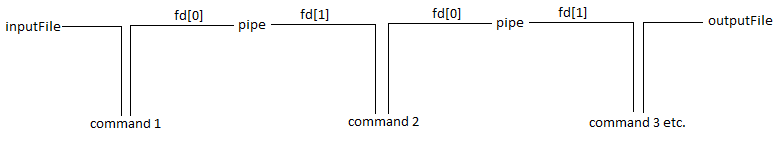
\includegraphics[scale=0.7, trim= 2cm 0cm 0cm 0cm]{pipefig}
\caption{En simpel figur over hvordan der pipes mellem de forskellige kommandoer og in- og output filerne.}
\label{fig:pipe}
\end{figure}
\vspace{1cm}

Vi valgte at udføre kommandoerne i den rækkefølge som resultaterne skulle bruges.
Med andre ord, hvis kommando k1's output skal pipes til kommando k2's input, så skal kommando k1 startes før kommando k2.
Hovedårsagen til dette valg var, at det gjorde det nemt at køre en kommando-række enten som forgrunds- eller baggrundsprocesser, da kommandoerne bare kan udføres, uden at hovedprocessen venter på en forgrundsproces, der venter på input. For at kunne have samtidig kørsel af kommandoer, der undervejs generere output, der pipes, så kan kun den sidste kommando køres som forgrundsproces. Det har medført, at hvis den sidste kommando terminerer før de forudgående baggrundsprocesser, kan det ske, at baggrundsprocesser efterlades kørende. Vi er nået frem til, at det er årsagen til, at kommando-listen oprindeligt vendte som den gjorde - med den sidste kommando først. Disse baggrundsprocesser er dog ikke synlige for brugeren, men det er muligivis stadigvæk problematisk, hvis en af de efterladte baggrundsprocessor ender i et deadlock, da det er usynligt for brugeren, hvilket ikke ville forventes med forgrundsprocesser.
